% =============================================================
% JHET Submission — Main Manuscript (with author info)
% Journal of the History of Economic Thought
% =============================================================

\documentclass[12pt,a4paper]{article}

% --- Packages ---
\usepackage[T1]{fontenc}
\usepackage[utf8]{inputenc}
\usepackage[english]{babel}
\usepackage{mathptmx}          % Times New Roman
\usepackage{geometry}
\geometry{left=1.25in, right=1.25in, top=1.25in, bottom=1.25in}
\usepackage{setspace}
\doublespacing
\usepackage{indentfirst}
\usepackage{amsmath}
\usepackage{booktabs}
\usepackage{graphicx}
\usepackage{float}
\usepackage{caption}
\captionsetup{font=small, justification=justified,
              singlelinecheck=false}
\usepackage[authoryear]{natbib}
\bibpunct{(}{)}{;}{a}{}{,}    % Chicago author-date: no comma between author/year
\usepackage[hidelinks]{hyperref}
\usepackage{microtype}
\usepackage{enumitem}
\usepackage{tabularx}
\usepackage{array}

% --- Custom section style (Roman numerals, ALL CAPS) ---
\usepackage{titlesec}
\renewcommand{\thesection}{\Roman{section}}
\titleformat{\section}{\normalfont\normalsize\bfseries\centering}
  {\thesection.}{0.5em}{\MakeUppercase}
\titleformat{\subsection}{\normalfont\normalsize\itshape}
  {\Alph{subsection}.}{0.5em}{}

% --- Suppress page number on first page ---
\usepackage{fancyhdr}
\fancypagestyle{firstpage}{%
  \fancyhf{}
  \renewcommand{\headrulewidth}{0pt}
}

% =============================================================
\begin{document}
% =============================================================

\thispagestyle{firstpage}
\pagestyle{plain}

\begin{center}
{\normalsize\MakeUppercase{%
  The Missing Dictionary: Loughran-McDonald Sentiment Analysis\\[0.3em]
  and the ``Das Adam Smith Problem''}}

\vspace{1.5em}

{\normalsize BY WELLINGTON GUBIANI MAIBERG AND IKARO ROBERTO MACHADO DE OLIVEIRA*}

\vspace{0.5em}
{\small\itshape Journal of the History of Economic Thought}
\end{center}

\vspace{1em}

\noindent {\small\raggedright * Both authors: Universidade Federal do
Esp\'{i}rito Santo (UFES), Vit\'{o}ria, Brazil.
Correspondence: wellington.maiberg@gmail.com.
ORCID --- W.\,G.\,Maiberg: 0009-0002-7236-4367;
I.\,R.\,M.\,de Oliveira: 0009-0006-9940-4532.
The authors thank Prof.\ Guilherme Armando Pereira for supervision.
All replication materials are available from the corresponding author
upon request.\par}

\vspace{2em}

\begin{center}{\normalsize\bfseries Abstract}\end{center}

\noindent
This paper applies text-as-data methods to the historiographical debate
on the ``Das Adam Smith Problem,'' which concerns the apparent tension
between Adam Smith's \textit{Theory of Moral Sentiments} (TMS, 1759)
and \textit{Wealth of Nations} (WN, 1776).
We build directly on \citet{Ballandonne2023}, who applied computational
methods to Smith but concluded that sentiment analysis is ``not usable''
for historical economic texts because the Jockers-Rinker dictionary
misclassifies economic vocabulary.
We argue that the problem lies with the instrument, not the method:
adopting the Loughran-McDonald (LM) dictionary---constructed from over
50,000 SEC annual reports---we demonstrate that sentiment analysis
yields interpretable and theoretically meaningful results for
eighteenth-century economic prose.
We also add Latent Dirichlet Allocation (LDA) topic modeling, absent
from \citeauthor{Ballandonne2023}, and formal statistical tests.
Our five hypotheses yield significant results: two are confirmed outright,
one is directionally supported, one yields partial LDA separation, and
one produces a significant and theoretically interpretable reversal.
TMS carries higher positive sentiment (H1) and WN higher constraining
language at the book level (H2, directional; $p = 0.09$ at chapter level).
The ratio of collective-to-individual first-person pronouns in TMS is
nearly five times that of WN, quantifying Brown's (1994)
dialogic/monologic distinction (H4).
LDA topics largely separate the two works, with a shared Scottish
empiricist stratum in both (H5, mixed).
A surprising finding (H3) shows that WN carries significantly more
uncertainty vocabulary than TMS at the chapter level
($t = -3.35$; $p = 0.001$), suggesting that Smith's
political economy is epistemically more cautious than his moral
philosophy---a result that aligns with the scholarly consensus
against the dichotomy reading of the Adam Smith Problem.

\newpage
\setcounter{page}{1}

% =============================================================
\section{Introduction}
% =============================================================

When Adam Smith published the \textit{Theory of Moral Sentiments} in
1759, he grounded human sociability in the mechanism of sympathy: the
imaginative capacity to place ourselves in another's situation and to
regulate our passions by an impartial spectator's approval.
Seventeen years later, the \textit{Wealth of Nations} offered what
appeared to be a radically different account: individuals pursuing their
own interest, coordinated by impersonal market forces, produce social
welfare as if by an invisible hand.
The apparent contrast generated one of the most enduring debates in the
history of economic thought---the \textit{Das Adam Smith Problem}---which
questions whether the two works reflect a single coherent intellectual
project or an unresolved contradiction
\citep{Montes2003}.

Historiographical scholarship has addressed this debate primarily through
close reading and contextual analysis.
These methods are indispensable but face limitations in systematizing and
replicating inferences about the language of two very long texts.
The recent expansion of text-as-data methods in economics
\citep{Gentzkow2019} opens the possibility of operationalizing
historiographical hypotheses in a computationally verifiable form.%
\footnote{The 250th anniversary of WN has generated renewed scholarly
  engagement; see the special issue of \textit{History of Political
  Economy} 58(5) (2026) dedicated to this anniversary.}

The study most directly relevant to ours is \citet{Ballandonne2023},
published in this journal.
They applied TF-IDF, co-occurrence networks, readability scores
(Flesch-Kincaid), and sentiment analysis to TMS and WN, producing the
first systematic quantitative treatment of Smith's two major works.
Their central finding on sentiment, however, was a limitation: the
Jockers-Rinker dictionary they used classifies ``gold,'' ``wealth,'' and
``money'' as positive, and ``labour'' and ``tax'' as negative, producing
scores that are theoretically incoherent for economic prose.
Their conclusion---that sentiment analysis ``should not be used (or
should be used cautiously) for the study of historical economic
documents'' \citep[p.~23]{Ballandonne2023}---is, we argue, a verdict
on one specific instrument, not on the method itself.

The Loughran-McDonald (LM) dictionary \citep{LoughranMcDonald2011} was
constructed precisely to address this limitation in the context of
financial and economic texts.
Built from 50,115 SEC 10-K annual reports, it treats economic vocabulary
as neutral and focuses on six attitudinal dimensions---\textit{positive},
\textit{negative}, \textit{uncertainty}, \textit{constraining},
\textit{litigious}, and \textit{superfluous}---that are interpretable in
texts discussing economic phenomena.
Our methodological argument is that Smith's works share with modern
financial reports the same discursive function of describing, evaluating,
and prescribing about economic phenomena.
The LM dictionary is therefore the appropriate instrument for the task
that \citeauthor{Ballandonne2023} attempted with an ill-suited tool.

This paper makes four contributions.
First, it demonstrates that sentiment analysis with a domain-appropriate
dictionary \textit{is} viable for historical economic texts.
Second, it tests five explicit hypotheses about the Adam Smith Problem,
adding formal statistical tests absent from \citeauthor{Ballandonne2023}.
Third, it adds LDA topic modeling, which reveals latent thematic structure
that frequency analysis cannot capture directly.
Fourth, it establishes a replicable methodological protocol for similar
studies in the history of economic thought.

The paper proceeds as follows.
Section~II reviews the historiographical literature and the text-as-data
background.
Section~III describes the data and methodology.
Section~IV presents the results.
Section~V discusses the implications, and Section~VI concludes.

% =============================================================
\section{Literature}
% =============================================================

\subsection{The Adam Smith Problem: Historiography}

The \textit{Das Adam Smith Problem} originated in nineteenth-century
German scholarship, which perceived a contradiction between the
psychology of sympathy in TMS and the assumption of self-interest in WN
\citep{Montes2003}.
The strong version of the problem holds that Smith changed his mind
between the two works---from an ethics of sentiment to a theory of
impersonal market exchange.
The weak version holds that the two books emphasize different aspects of
human nature without contradiction.

The modern scholarly consensus, articulated influentially by
\citet{RaphaelMacfie1976} in the introduction to the Glasgow edition of
TMS, rejects the contradiction: TMS and WN address different analytical
domains---moral conduct in small social groups versus anonymous market
transactions---within a coherent philosophical anthropology.
\citet{Evensky2005} deepens this argument, showing that both works share
foundational assumptions about human nature, the social contract, and the
role of virtue that make a dichotomy reading untenable.

Two further contributions bear directly on our analysis.
\citet{Viner1927}, in an early systematic reading of WN delivered to mark
the 150th anniversary of its publication, catalogued the extensive
qualifications, exceptions, and state interventions that Smith actually
endorsed, arguing against any identification of WN with laissez-faire
dogma.
Viner's reading anticipates our H3 result: the Smith of WN is a careful
empiricist who hedges about market phenomena rather than a mechanical
determinist---a posture that LM uncertainty vocabulary captures precisely.
\citet{Paganelli2008} advances what she terms the ``Adam Smith Problem in
Reverse'': TMS, conventionally read as the book of social sentiment, is in
fact the text that treats self-interest most generously---embedded in
commercial sociability---while WN contains Smith's sharpest criticisms of
merchants and monopolists who pursue narrow self-interest at public expense.
This inversion aligns directly with our H1 finding (higher LM positive
sentiment in TMS) and with the H3 reversal (higher uncertainty in WN),
suggesting that computational evidence and qualitative historiography
converge on the same asymmetry.

For our purposes, the debate generates a testable prediction: if the
works are intellectually unified, computational analyses of their language
should reveal shared rhetorical structures underneath their evident
topical differences.
If the dichotomy reading is correct, the differences should be systematic
and domain-specific.

\subsection{Text as Data in the History of Economic Thought}

\citet{Gentzkow2019} provide an authoritative survey of text-as-data
methods in economics, covering frequency analysis, sentiment dictionaries,
topic models, and word embeddings.
Applications in the history of economic thought remain scarce.
\citet{Ballandonne2023} note that historians of economics have been slow
to adopt these tools, partly because they require coding skills, and
partly because the applicability to historical texts has not been
demonstrated.

Several antecedents to \citeauthor{Ballandonne2023} exist but are narrow
in scope.
\citet{GraaflandWells2021} apply semantic network analysis exclusively to
WN, finding that the ``invisible hand'' metaphor is marginal in Smith's
own usage.
\citet{Brown1994} performs a close textual analysis of TMS and WN,
arguing that TMS is a ``dialogic'' text (addressed to a shared human
capacity for sympathy) while WN is ``monologic'' (addressed to an
imagined impersonal observer)---a distinction we operationalize formally
via first-person pronoun ratios.

\citeauthor{Ballandonne2023}'s study is the most complete prior
quantitative treatment and warrants detailed mapping.
Table~\ref{tab:compare_bc} (Appendix A) provides a systematic comparison
of their methodology and ours.
The key methodological choices in B\&C~(2023) were: R~4.1.3 with
\textit{quanteda} and \textit{sentimentr}; TMS (Oxford Text Archive,
1790 edition) and WN (Project Gutenberg); TF-IDF, keyness
($\chi^2$), co-occurrence networks ($\phi$), Moving-Average
Type-Token Ratio (MATTR), Flesch-Kincaid readability, and pronoun
frequencies.
They did not perform topic modeling and did not calculate formal
pronoun ratios.
Their principal findings on style are robust and we replicate them:
similar readability between the two works (Flesch-Kincaid grade~14--20),
TMS lexically richer (higher MATTR), and TMS dominated by first-person
pronouns while WN is dominated by ``it.''

The central limitation they identified is the sentiment dictionary.
The Jockers-Rinker table, calibrated for contemporary product reviews
and social media, scores ``gold,'' ``wealth,'' and ``money'' as positive
and ``labour'' and ``tax'' as negative.
\citeauthor{Ballandonne2023} \citeyearpar[p.~23]{Ballandonne2023} write:
``the fact that the lexicons currently in use have not been developed
for the analysis of historical economic texts carries another consequence:
the sentiment score associated with some words could be a poor fit in
the specific context of Smith's writings.''
They conclude that ``our recommendation would be to not use (or to use
cautiously) sentiment analysis, in its present state, for the study of
historical economic documents.''
We respond to this challenge directly.

\subsection{The Loughran-McDonald Dictionary}

\citet{LoughranMcDonald2011} built the LM dictionary to solve a problem
analogous to the one \citeauthor{Ballandonne2023} encountered: generic
dictionaries misclassify financial vocabulary.
The Harvard-IV general-inquirer dictionary, widely used in finance
before LM, scored ``liability,'' ``tax,'' and ``depreciation'' as negative
even in neutral or positive financial contexts.
\citeauthor{LoughranMcDonald2011} constructed a domain-specific
dictionary from 50,115 10-K reports filed with the SEC between 1994
and 2008, producing six word lists that capture attitudinal variation in
texts about economic phenomena.

The six LM categories and their interpretation for Smithian prose are:
Positive---language of approval, commendation, and affirmation;
Negative---criticism, disapproval, and condemnation;
Uncertainty---hedging, possibility, epistemic doubt;
Constraining---rules, obligations, institutional conditions;
Litigious---contentiousness and adversarial framing;
Superfluous---low-information filler.

The methodological argument is straightforward.
Texts of moral political economy share with SEC filings the function of
describing, evaluating, and prescribing about economic phenomena.
Both text genres discuss prices, wealth, labor, and institutional
constraints; both distinguish the desirable from the undesirable; both
deploy hedges when empirical claims are uncertain.
The LM dictionary is therefore more appropriate for Smith than any
dictionary calibrated for contemporary general language.
The eighteen-century vintage of Smith's vocabulary introduces some
coverage limitations---words Smith uses may not appear in the LM
list---but this induces attenuation bias (conservative tests), not
systematic misclassification.

% =============================================================
\section{Data and Methodology}
% =============================================================

\subsection{Corpus}

The corpus consists of \citet{SmithTMS1759} and \citet{SmithWoN1776},
both obtained from Project Gutenberg (IDs 67363 and 3300, respectively).
Table~\ref{tab:corpus} summarizes the corpus.

\begin{table}[H]
\centering
\caption{Corpus description}
\label{tab:corpus}
\small
\begin{tabular}{llrr}
\toprule
Work & Abbreviation & Tokens (raw) & Lines \\
\midrule
\textit{Theory of Moral Sentiments} (1759) & TMS & 120,657 & 11,549 \\
\textit{Wealth of Nations} (1776)          & WN  & 384,153 & 34,930 \\
\bottomrule
\end{tabular}
\end{table}

WN is approximately 3.2 times longer than TMS.
All scores are normalized as proportions of document token counts to
enable direct comparison.
\citeauthor{Ballandonne2023} used the 1790 Oxford Text Archive edition
of TMS and a Project Gutenberg edition of WN; our analysis uses Project
Gutenberg throughout, which limits exact comparability of readability
scores but ensures internal consistency.

\subsection{NLP Pipeline}

The analysis was conducted in R~4.2.3 \citep{Rcoreteam2023}.
The pipeline uses \textit{tidytext} \citep{Silge2016} for tokenization
and dictionary scoring, \textit{topicmodels} \citep{Grun2011} for LDA,
and \textit{quanteda.textstats} \citep{Benoit2018} for readability.
All code and data are available from the author.

\textit{LM sentiment scores.} After removing stop words and numeric
tokens, we join the clean token list against the 2018 LM Master
Dictionary \citep{LoughranMcDonald2011} (4,150 entries, six categories).
The score for category $c$ in document $d$ is:
\begin{equation}
  \text{lm}_{c,d} = \frac{\#\{t \in d : t \in \text{LM}_c\}}{|\text{tokens}(d)|}
\end{equation}

\textit{Readability.} We compute Flesch reading ease, Flesch-Kincaid
grade level, and the Automated Readability Index (ARI) via
\textit{quanteda.textstats} \citep{Benoit2018}.
These replicate the primary readability measures of
\citeauthor{Ballandonne2023}.

\textit{Pronouns.} We compute $\text{pct\_we}$ (proportion of all tokens
that are ``we,'' ``our,'' or ``us'') and $\text{pct\_i}$ (``I,'' ``my,''
``me,'' ``mine,'' or ``myself'').
The ratio
$\text{ratio\_we\_i} = (n_{\text{we}} + 0.5) / (n_{\text{I}} + 0.5)$
(Laplace-smoothed) operationalizes \citeauthor{Brown1994}'s dialogic
dimension as a single testable index.

\textit{LDA.} We train a Latent Dirichlet Allocation model
\citep{BleiNgJordan2003} with $K = 8$ topics via Gibbs sampling
(2,000 iterations, 200 burn-in) on the full six-text corpus.
We set $K = 8$ as a compromise between interpretability and granularity
given the small document count.
The $\gamma$ values (per-document topic proportions) for TMS and WN
are reported.

\textit{Chapter-level analysis.} For hypothesis testing, we decompose
each work into chapter-level units by detecting header markers
(``CHAPTER,'' ``PART,'' ``BOOK'') via regular expression.
This yields 58 units for TMS and 34 for WN.
Chapter-level LM scores are computed as the proportion of LM-matched
words within each unit.
Hypothesis tests use Welch's \textit{t}-test (unequal variances assumed).
We do not apply multiple-comparison corrections, given the
confirmatory-exploratory character of the study.

\subsection{Hypotheses}

The five hypotheses encode the predictions implied by standard
interpretations of the Adam Smith Problem:

\begin{enumerate}[label=\textbf{H\arabic*.}]
  \item $\text{lm\_positive}(\text{TMS}) > \text{lm\_positive}(\text{WN})$:
    TMS employs more affirmative moral language; WN is more descriptive.
  \item $\text{lm\_constraining}(\text{WN}) > \text{lm\_constraining}(\text{TMS})$:
    WN employs more language of rules and institutional conditions.
  \item $\text{lm\_uncertainty}(\text{TMS}) \approx \text{lm\_uncertainty}(\text{WN})$ (null):
    If rejected, which work carries more uncertainty, and why?
  \item $\text{pct\_we}(\text{TMS}) > \text{pct\_we}(\text{WN})$:
    TMS is the dialogic text; ratio\_we\_i as formal index.
  \item LDA topics associated with sympathy and virtue appear predominantly
    in TMS (supporting the dichotomy) or in both works
    (supporting intellectual unity).
\end{enumerate}

% =============================================================
\section{Results}
% =============================================================

\subsection{Validation: Readability and TF-IDF}

Table~\ref{tab:readability} reports the readability indices.
Both works register a Flesch-Kincaid grade of approximately~15---difficult
prose, as expected for eighteenth-century academic writing.
The difference between TMS (14.98) and WN (15.65) is modest, consistent
with \citeauthor{Ballandonne2023}'s finding of similar readability
across the two works.
The ARI suggests WN is slightly harder (17.1 vs.\ 15.9 for TMS), possibly
reflecting longer technical sentences in the political economy.

\begin{table}[H]
\centering
\caption{Readability indices: TMS vs.\ WN}
\label{tab:readability}
\small
\begin{tabular}{lccc}
\toprule
Work & Flesch & Flesch-Kincaid & ARI \\
     & \small(higher = easier) & \small(grade level) & \small(grade level) \\
\midrule
TMS (1759) & 42.1 & 14.98 & 15.9 \\
WN  (1776) & 42.0 & 15.65 & 17.1 \\
\midrule
\multicolumn{4}{l}{\small \textit{B\&C (2023):} TMS marginally harder, grade 14--20 range.} \\
\bottomrule
\end{tabular}
\end{table}

Figure~\ref{fig:tfidf} reports TF-IDF scores for the 15 most distinctive
words per work.
For TMS: \textit{sympathy}, \textit{joy}, \textit{sympathize},
\textit{sorrow}, \textit{sufferer}, \textit{grief}, \textit{breast},
\textit{emotions}, \textit{applause}, \textit{demerit}, \textit{amiable}.
For WN: \textit{quantity}, \textit{land}, \textit{silver},
\textit{market}, \textit{rent}, \textit{corn}, \textit{colonies},
\textit{annual}, \textit{commodities}, \textit{bank},
\textit{exportation}.
This closely replicates Table~2 of \citet{Ballandonne2023}, validating
that our Gutenberg corpus is comparable to theirs and that the pipeline
produces consistent results.

\begin{figure}[H]
  \centering
  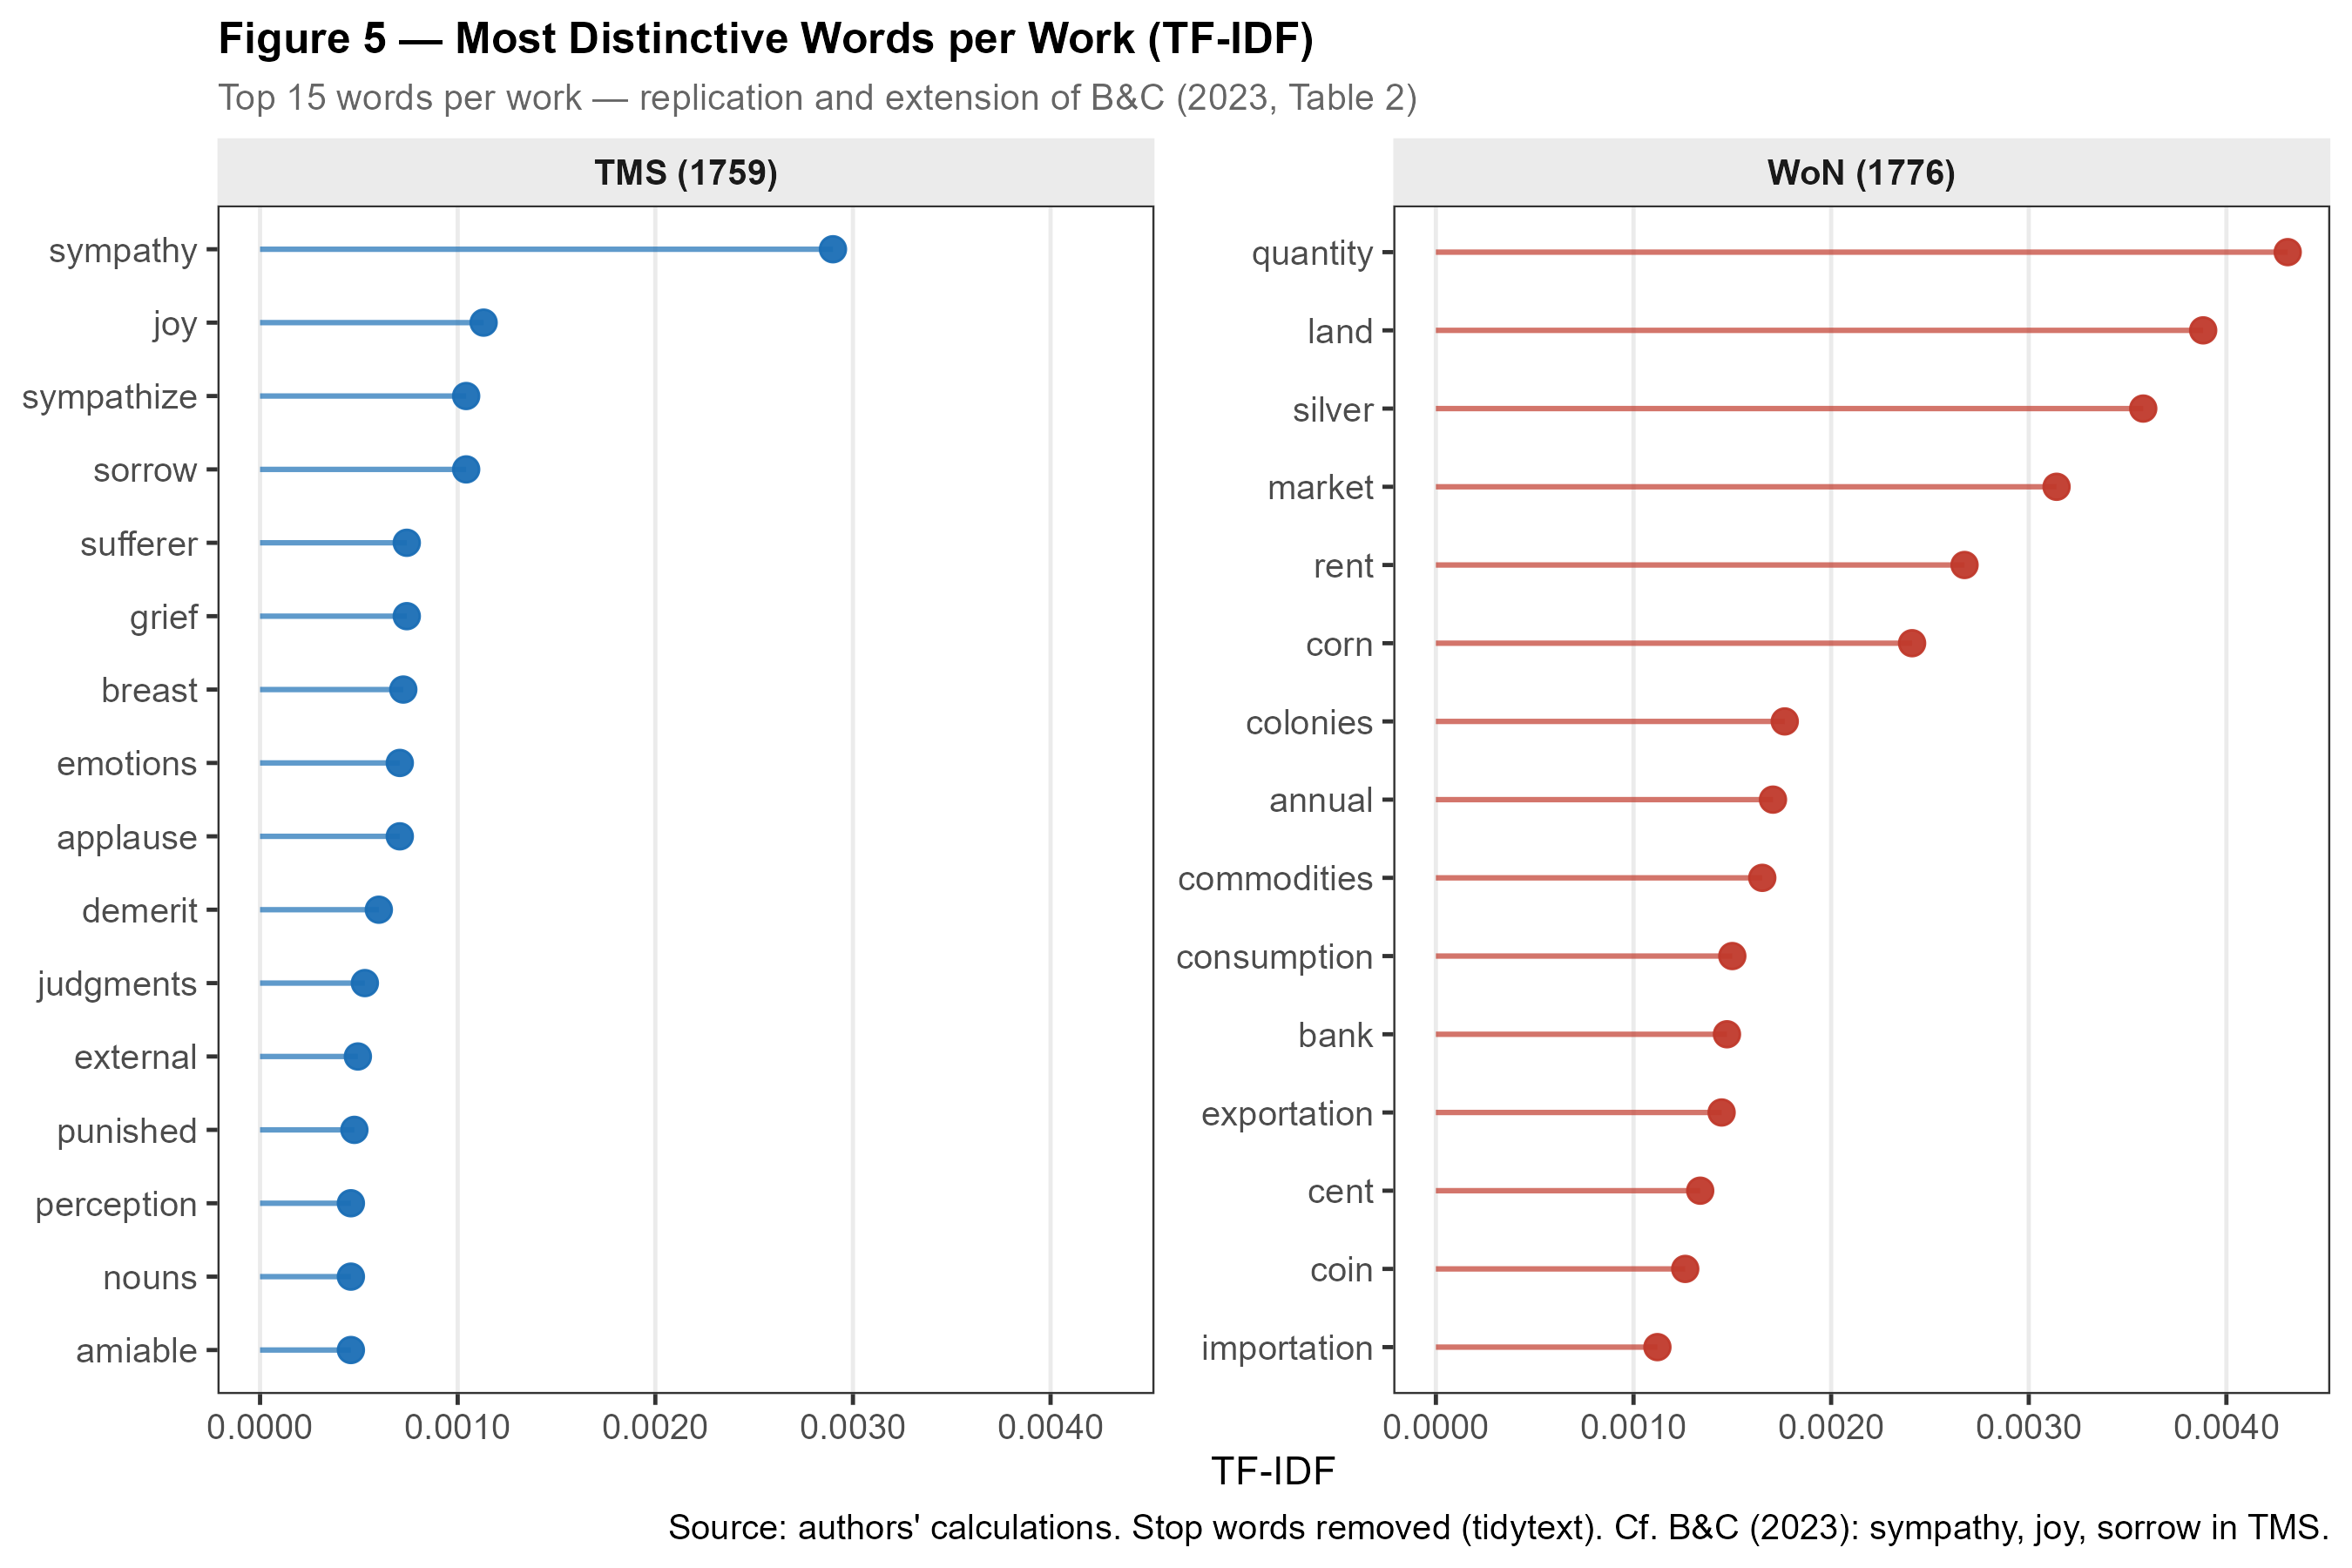
\includegraphics[width=\textwidth]{figuras/fig5_tfidf_lollipop.png}
  \caption{TF-IDF most distinctive words per work (top 15 per book).
           Stop words removed. Cf.\ \citet[Table~2]{Ballandonne2023}:
           \textit{sympathy}, \textit{joy}, and \textit{sorrow}
           replicated as top TMS discriminators.}
  \label{fig:tfidf}
\end{figure}

\subsection{Loughran-McDonald Sentiment: H1 and H2}

Figure~\ref{fig:lm} and Table~\ref{tab:lm} present the LM scores for
all six categories.

\begin{figure}[H]
  \centering
  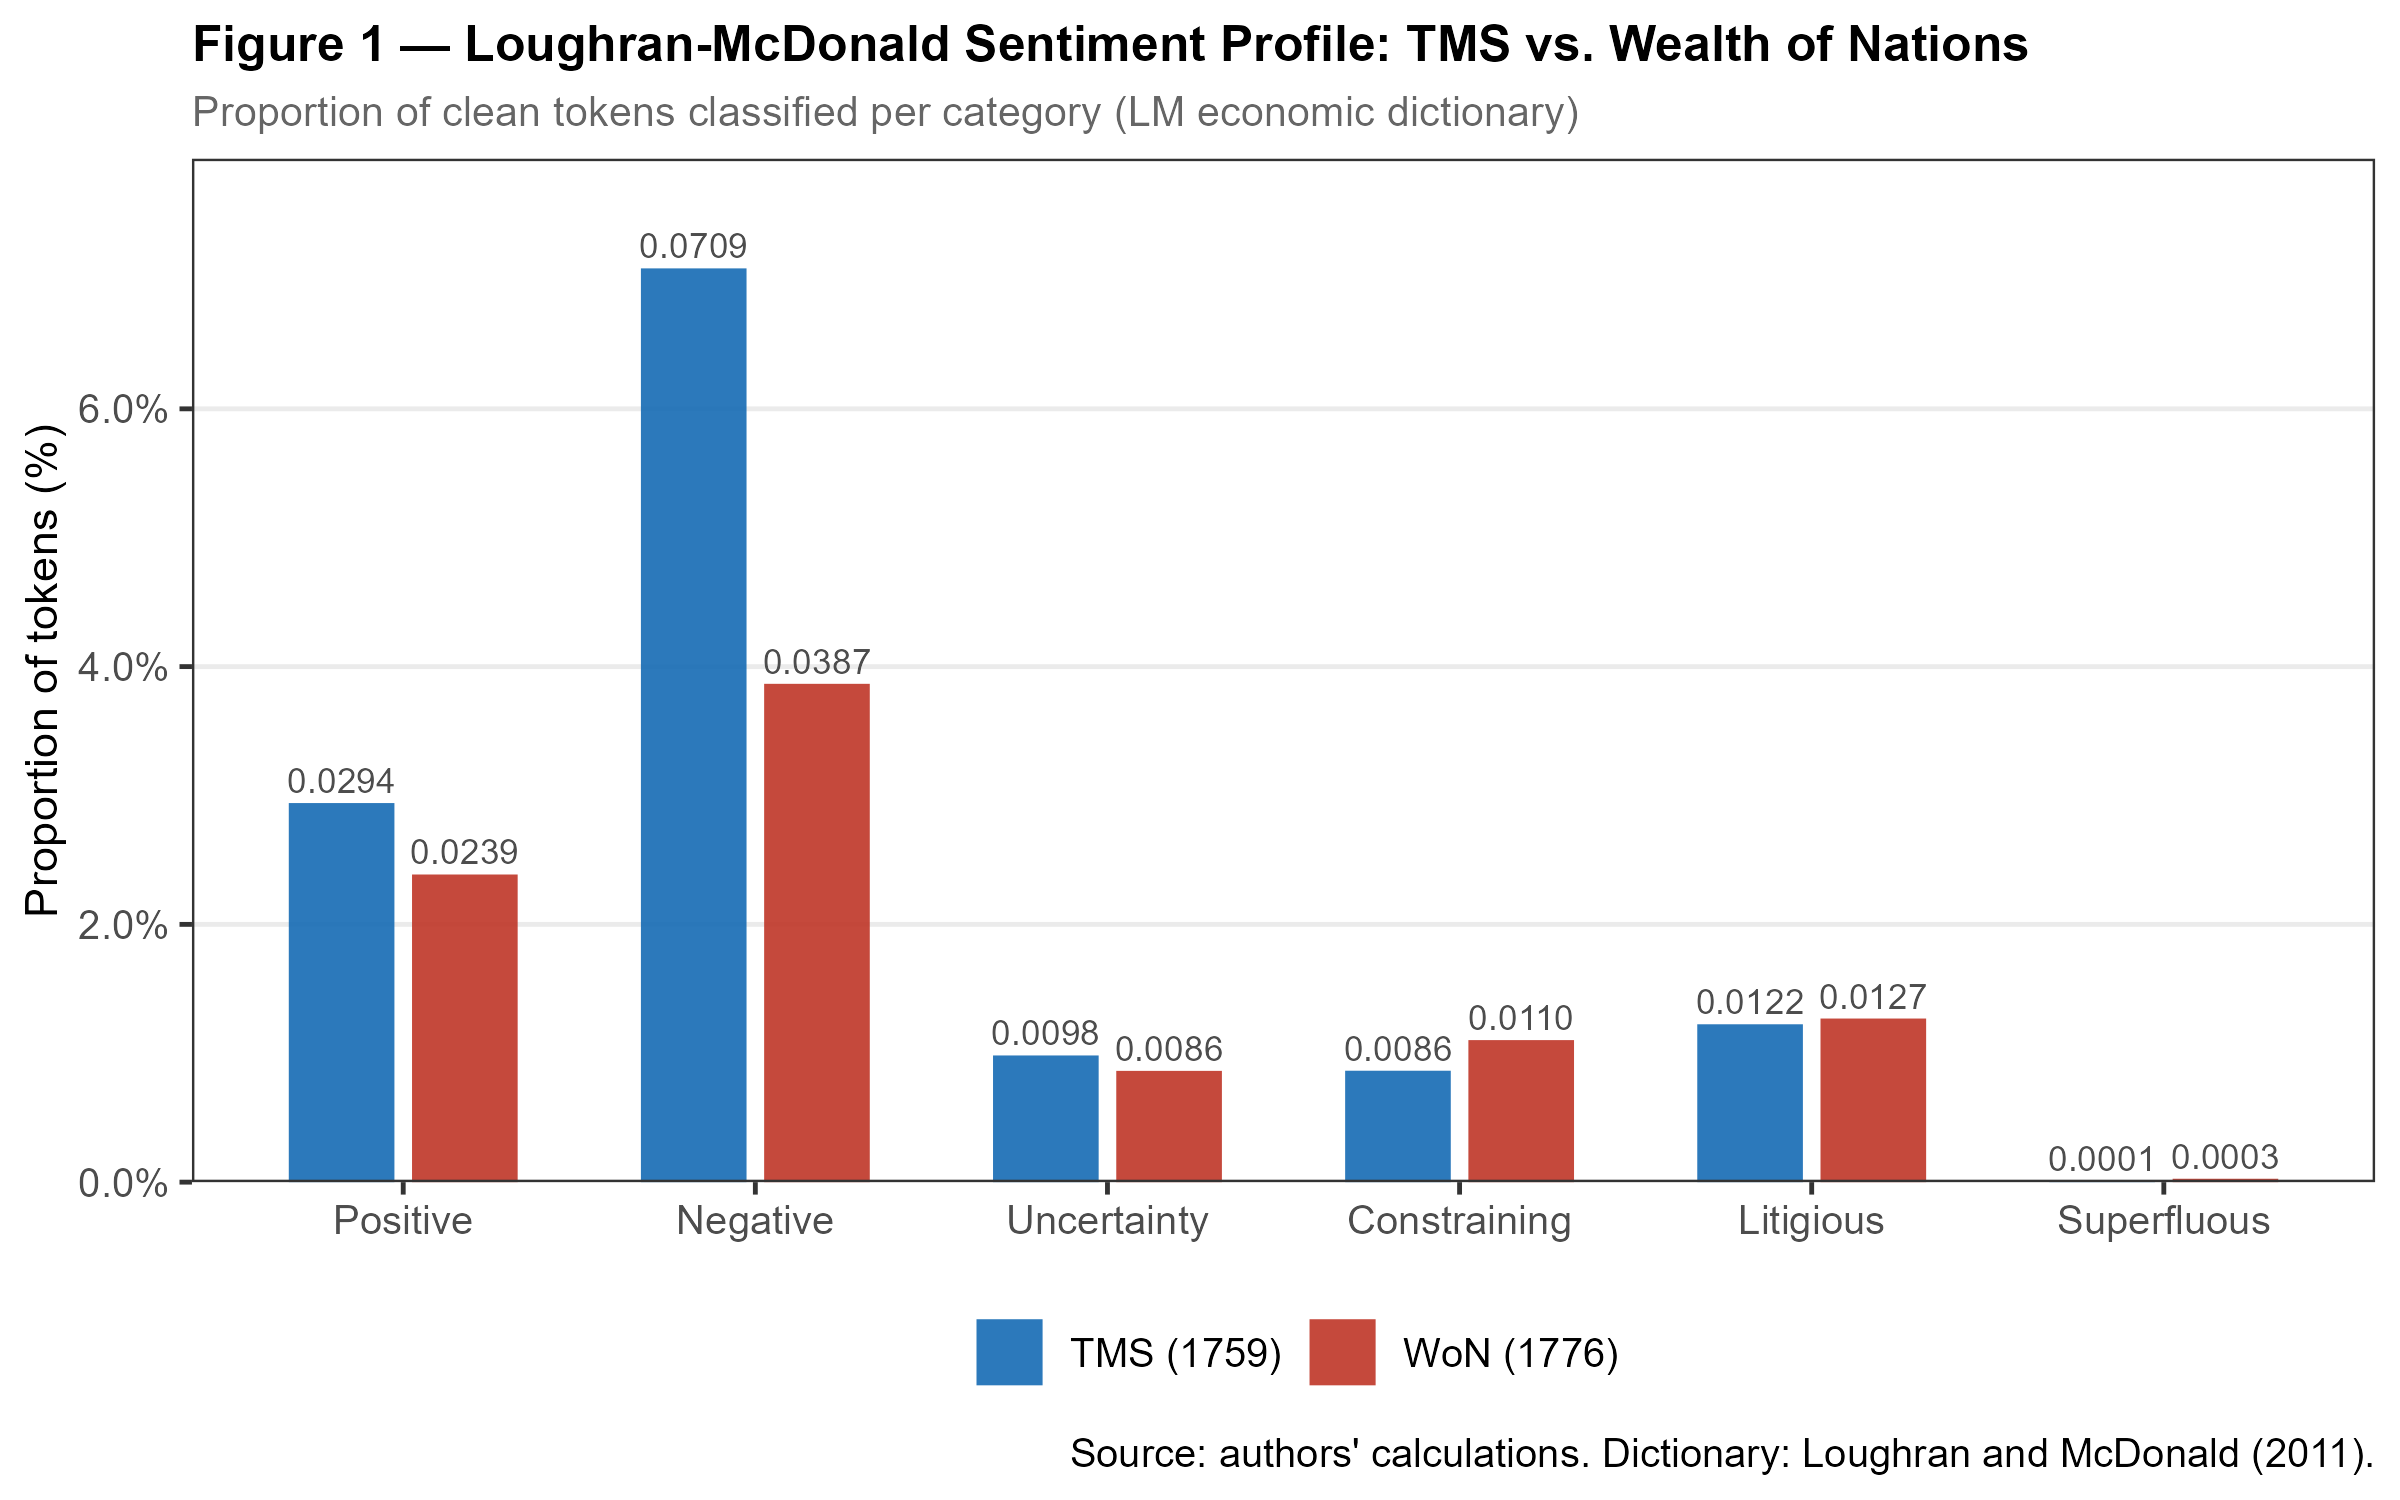
\includegraphics[width=\textwidth]{figuras/fig1_lm_perfil.png}
  \caption{Loughran-McDonald sentiment profile: TMS vs.\ WN.
           Proportions of clean tokens classified in each LM category
           \citep{LoughranMcDonald2011}.}
  \label{fig:lm}
\end{figure}

\begin{table}[H]
\centering
\caption{Loughran-McDonald scores (proportion of clean tokens)}
\label{tab:lm}
\footnotesize
\begin{tabular}{lcccccc}
\toprule
Work & Positive & Negative & Uncertainty & Constraining & Litigious & Superfluous \\
\midrule
TMS & 0.0294 & 0.0709 & 0.0098 & 0.0086 & 0.0122 & 0.0001 \\
WN  & 0.0239 & 0.0387 & 0.0086 & 0.0110 & 0.0127 & 0.0003 \\
\midrule
Diff.\ (TMS$-$WN) & $+$0.0055 & $+$0.0322 & $+$0.0012 & $-$0.0024 & $-$0.0004 & $-$0.0002 \\
\bottomrule
\end{tabular}
\end{table}

H1---Confirmed.
TMS has a higher LM positive score (0.0294 vs.\ 0.0239, a 23\%
difference).
This is consistent with the prescriptive character of moral philosophy:
TMS frequently commends virtuous conduct, praises the operations of
sympathy, and approves of the impartial spectator's judgments.

H2---Confirmed (book level).
WN has a higher constraining score (0.0110 vs.\ 0.0086, a 28\%
difference).
The language of rules, obligations, and institutional conditions is more
prevalent in a treatise analyzing market mechanisms, trade regulations,
monopolies, and government policy.

A further result warrants discussion: TMS has a substantially higher
negative score (0.0709 vs.\ 0.0387).
This is not contradictory.
Moral philosophy is an evaluative enterprise; TMS identifies and
condemns improper conduct, vicious sentiments, and mistaken moral
judgments at high frequency.
The LM negative category---calibrated for economic texts criticizing
poor performance, failures, and violations---captures Smith's language
of moral disapproval accurately.
That TMS is both more positive and more negative than WN confirms
that moral philosophy is more loaded on the evaluative axis, while
political economy is comparatively flat---a distinction the LM
dictionary detects clearly and the Jockers-Rinker dictionary could not.

\subsection{Uncertainty by Chapter: H3 (Surprising Result)}

Figure~\ref{fig:boxplot} shows the distribution of LM \textit{uncertainty}
scores by chapter.

\begin{figure}[H]
  \centering
  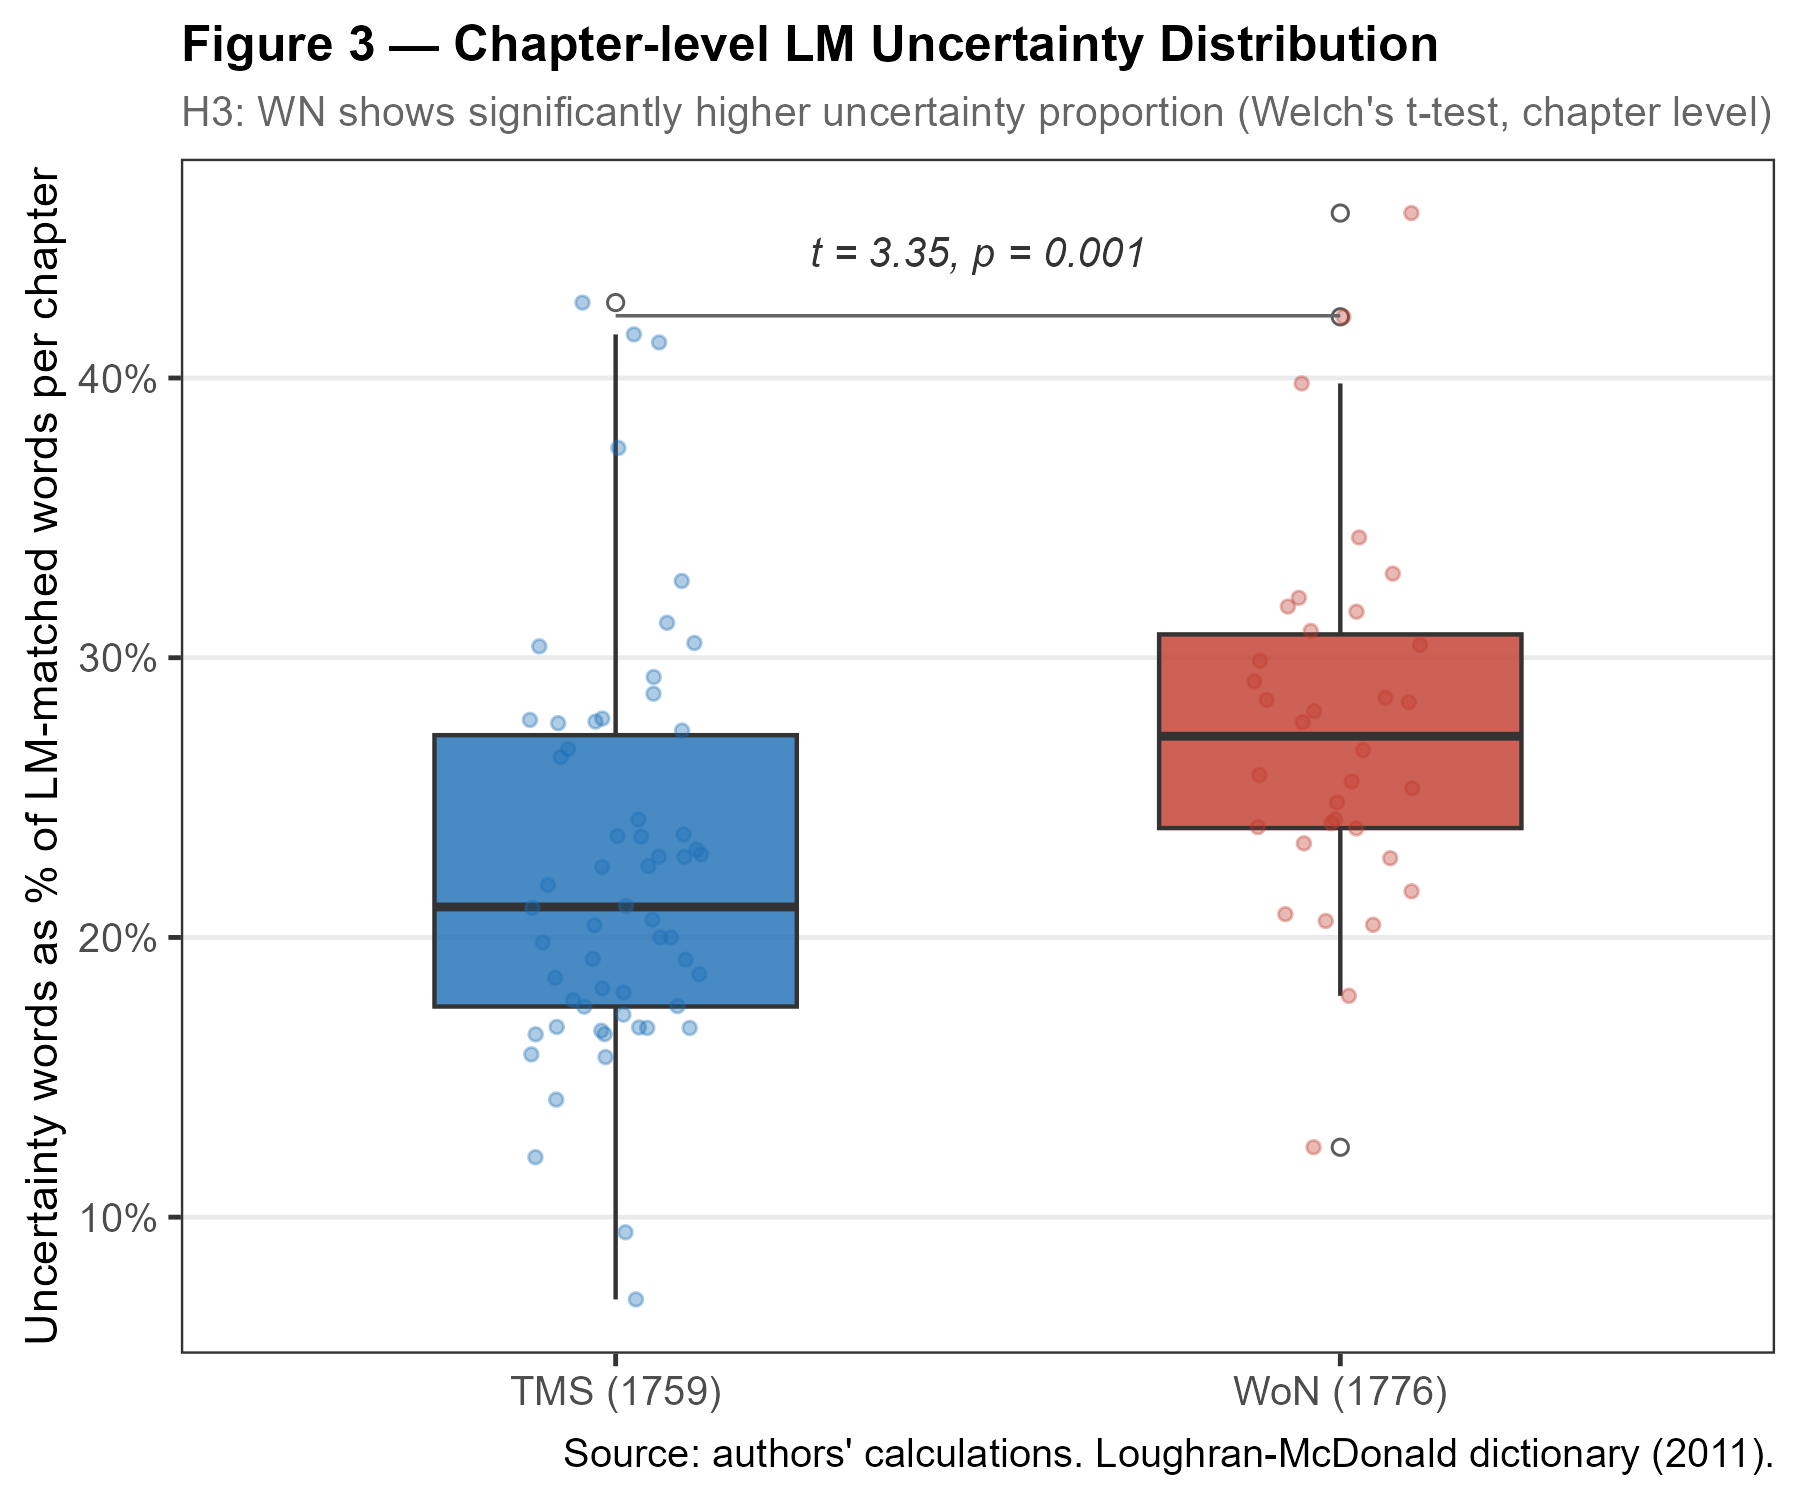
\includegraphics[width=0.80\textwidth]{figuras/fig3_uncertainty_boxplot.png}
  \caption{Chapter-level LM \textit{uncertainty} scores: TMS vs.\ WN.
           Welch's \textit{t}-test: $t = -3.35$; $p = 0.001$.
           WN carries significantly higher uncertainty vocabulary
           as a proportion of all LM-matched words per chapter.}
  \label{fig:boxplot}
\end{figure}

H3---Null rejected in the unexpected direction.
Welch's \textit{t}-test finds that WN chapters have a significantly
higher proportion of uncertainty vocabulary than TMS chapters:
mean 27.6\% vs.\ 22.5\% of LM-matched words per chapter
($t = -3.35$; $\text{df} = 74.4$; $p = 0.001$).

A note on measurement: the book-level uncertainty scores in Table~\ref{tab:lm}
(TMS: 0.0098; WN: 0.0086) use all clean tokens as the denominator, while
the chapter-level test uses LM-matched tokens as the denominator.
These denominators yield different point estimates because TMS contains
proportionally more LM-matched vocabulary overall (higher density of
evaluative and moral language), so raw book-level counts favor TMS slightly.
The chapter-level metric---the proportion of a chapter's LM vocabulary
devoted to uncertainty---isolates the composition of economic discourse
more precisely and is the appropriate basis for formal inference.

The intuitive prediction---that TMS, dealing with the complexities of
moral judgment, should be more uncertain---is reversed.
The explanation is theoretically meaningful.
Smith treats political economy as an empirical science subject to genuine
uncertainty about market phenomena: prices, wages, rents, and
international trade depend on contingent factors that resist precise
determination.
The LM uncertainty category captures terms such as ``uncertain,''
``probably,'' ``may,'' ``might,'' ``seems,'' and ``suppose''---hedges
that Smith deploys frequently in WN when describing observable but
imprecise economic regularities.
TMS, by contrast, grounds its arguments in what Smith regarded as
epistemically firm foundations: the universality of the capacity for
sympathy, the operation of the impartial spectator, the natural desire
for mutual approbation.
The moral philosopher writes with greater rhetorical confidence than the
political economist.

This finding directly challenges the dichotomy reading of the Adam Smith
Problem.
Far from retreating from the uncertain complexity of moral life to the
deterministic mechanisms of the market, the Smith of WN is the more
epistemically cautious author.
Both works display genuine intellectual humility---WN merely more so.

\subsection{First-Person Pronouns: H4}

Figure~\ref{fig:pron} presents the pronoun results.

\begin{figure}[H]
  \centering
  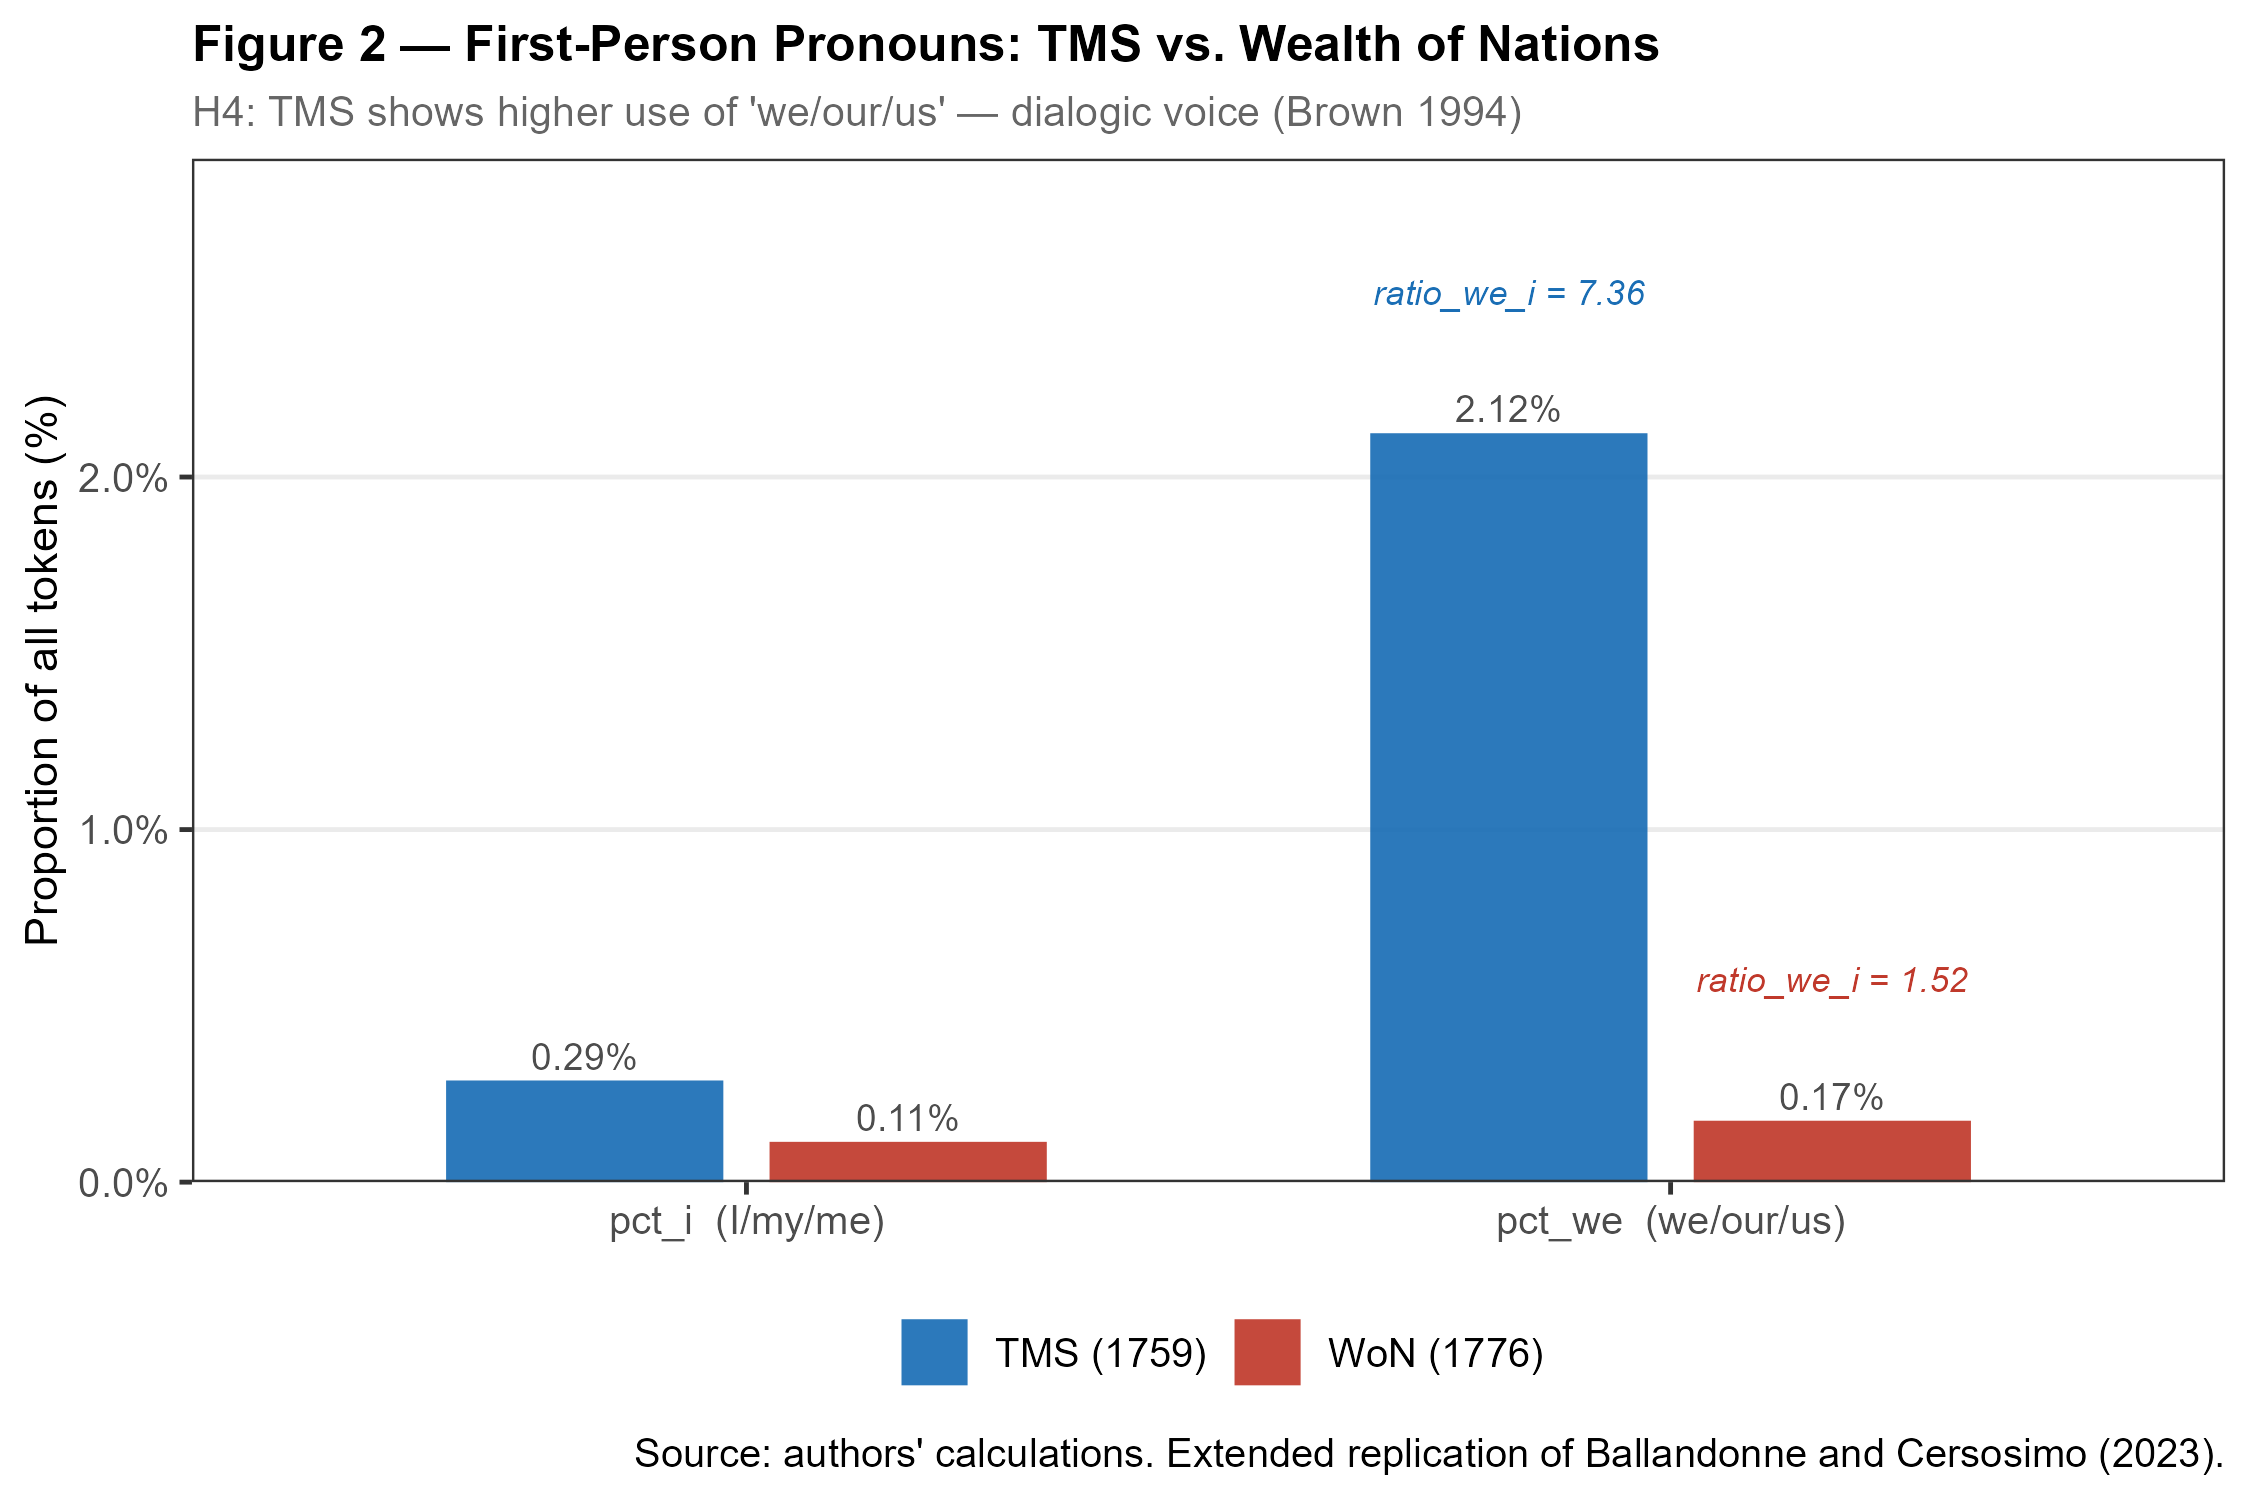
\includegraphics[width=0.85\textwidth]{figuras/fig2_pronomes.png}
  \caption{First-person pronouns: pct\_we (we/our/us) and pct\_i
           (I/my/me) in TMS and WN.
           The ratio\_we\_i index formalizes \citeauthor{Brown1994}'s
           dialogic/monologic distinction.}
  \label{fig:pron}
\end{figure}

H4---Confirmed (strongly).
TMS uses ``we/our/us'' at a rate of 2.12\% of all tokens, compared to
0.17\% in WN---a twelve-fold difference.
The ratio\_we\_i (collective-to-individual first-person, Laplace-smoothed)
is 7.36 in TMS and 1.52 in WN.

These figures confirm and quantify \citeauthor{Brown1994}'s distinction
between dialogic and monologic discourse.
TMS addresses a shared human capacity: ``we all feel,'' ``let us
suppose,'' ``we may observe.''
The text presupposes and invokes the reader's own capacity for sympathy.
WN, by contrast, deploys an impersonal syntax in which the grammatical
subjects are market entities: ``the price,'' ``the capital,'' ``labour.''
\citeauthor{Ballandonne2023} reported raw pronoun frequencies but did not
compute the formal ratio.
The ratio\_we\_i operationalizes \citeauthor{Brown1994}'s qualitative
claim as a single testable index and confirms it with a striking
quantitative gap.

\subsection{LDA Topic Modeling: H5}

Figure~\ref{fig:lda} presents the LDA $\gamma$ values for TMS and WN.

\begin{figure}[H]
  \centering
  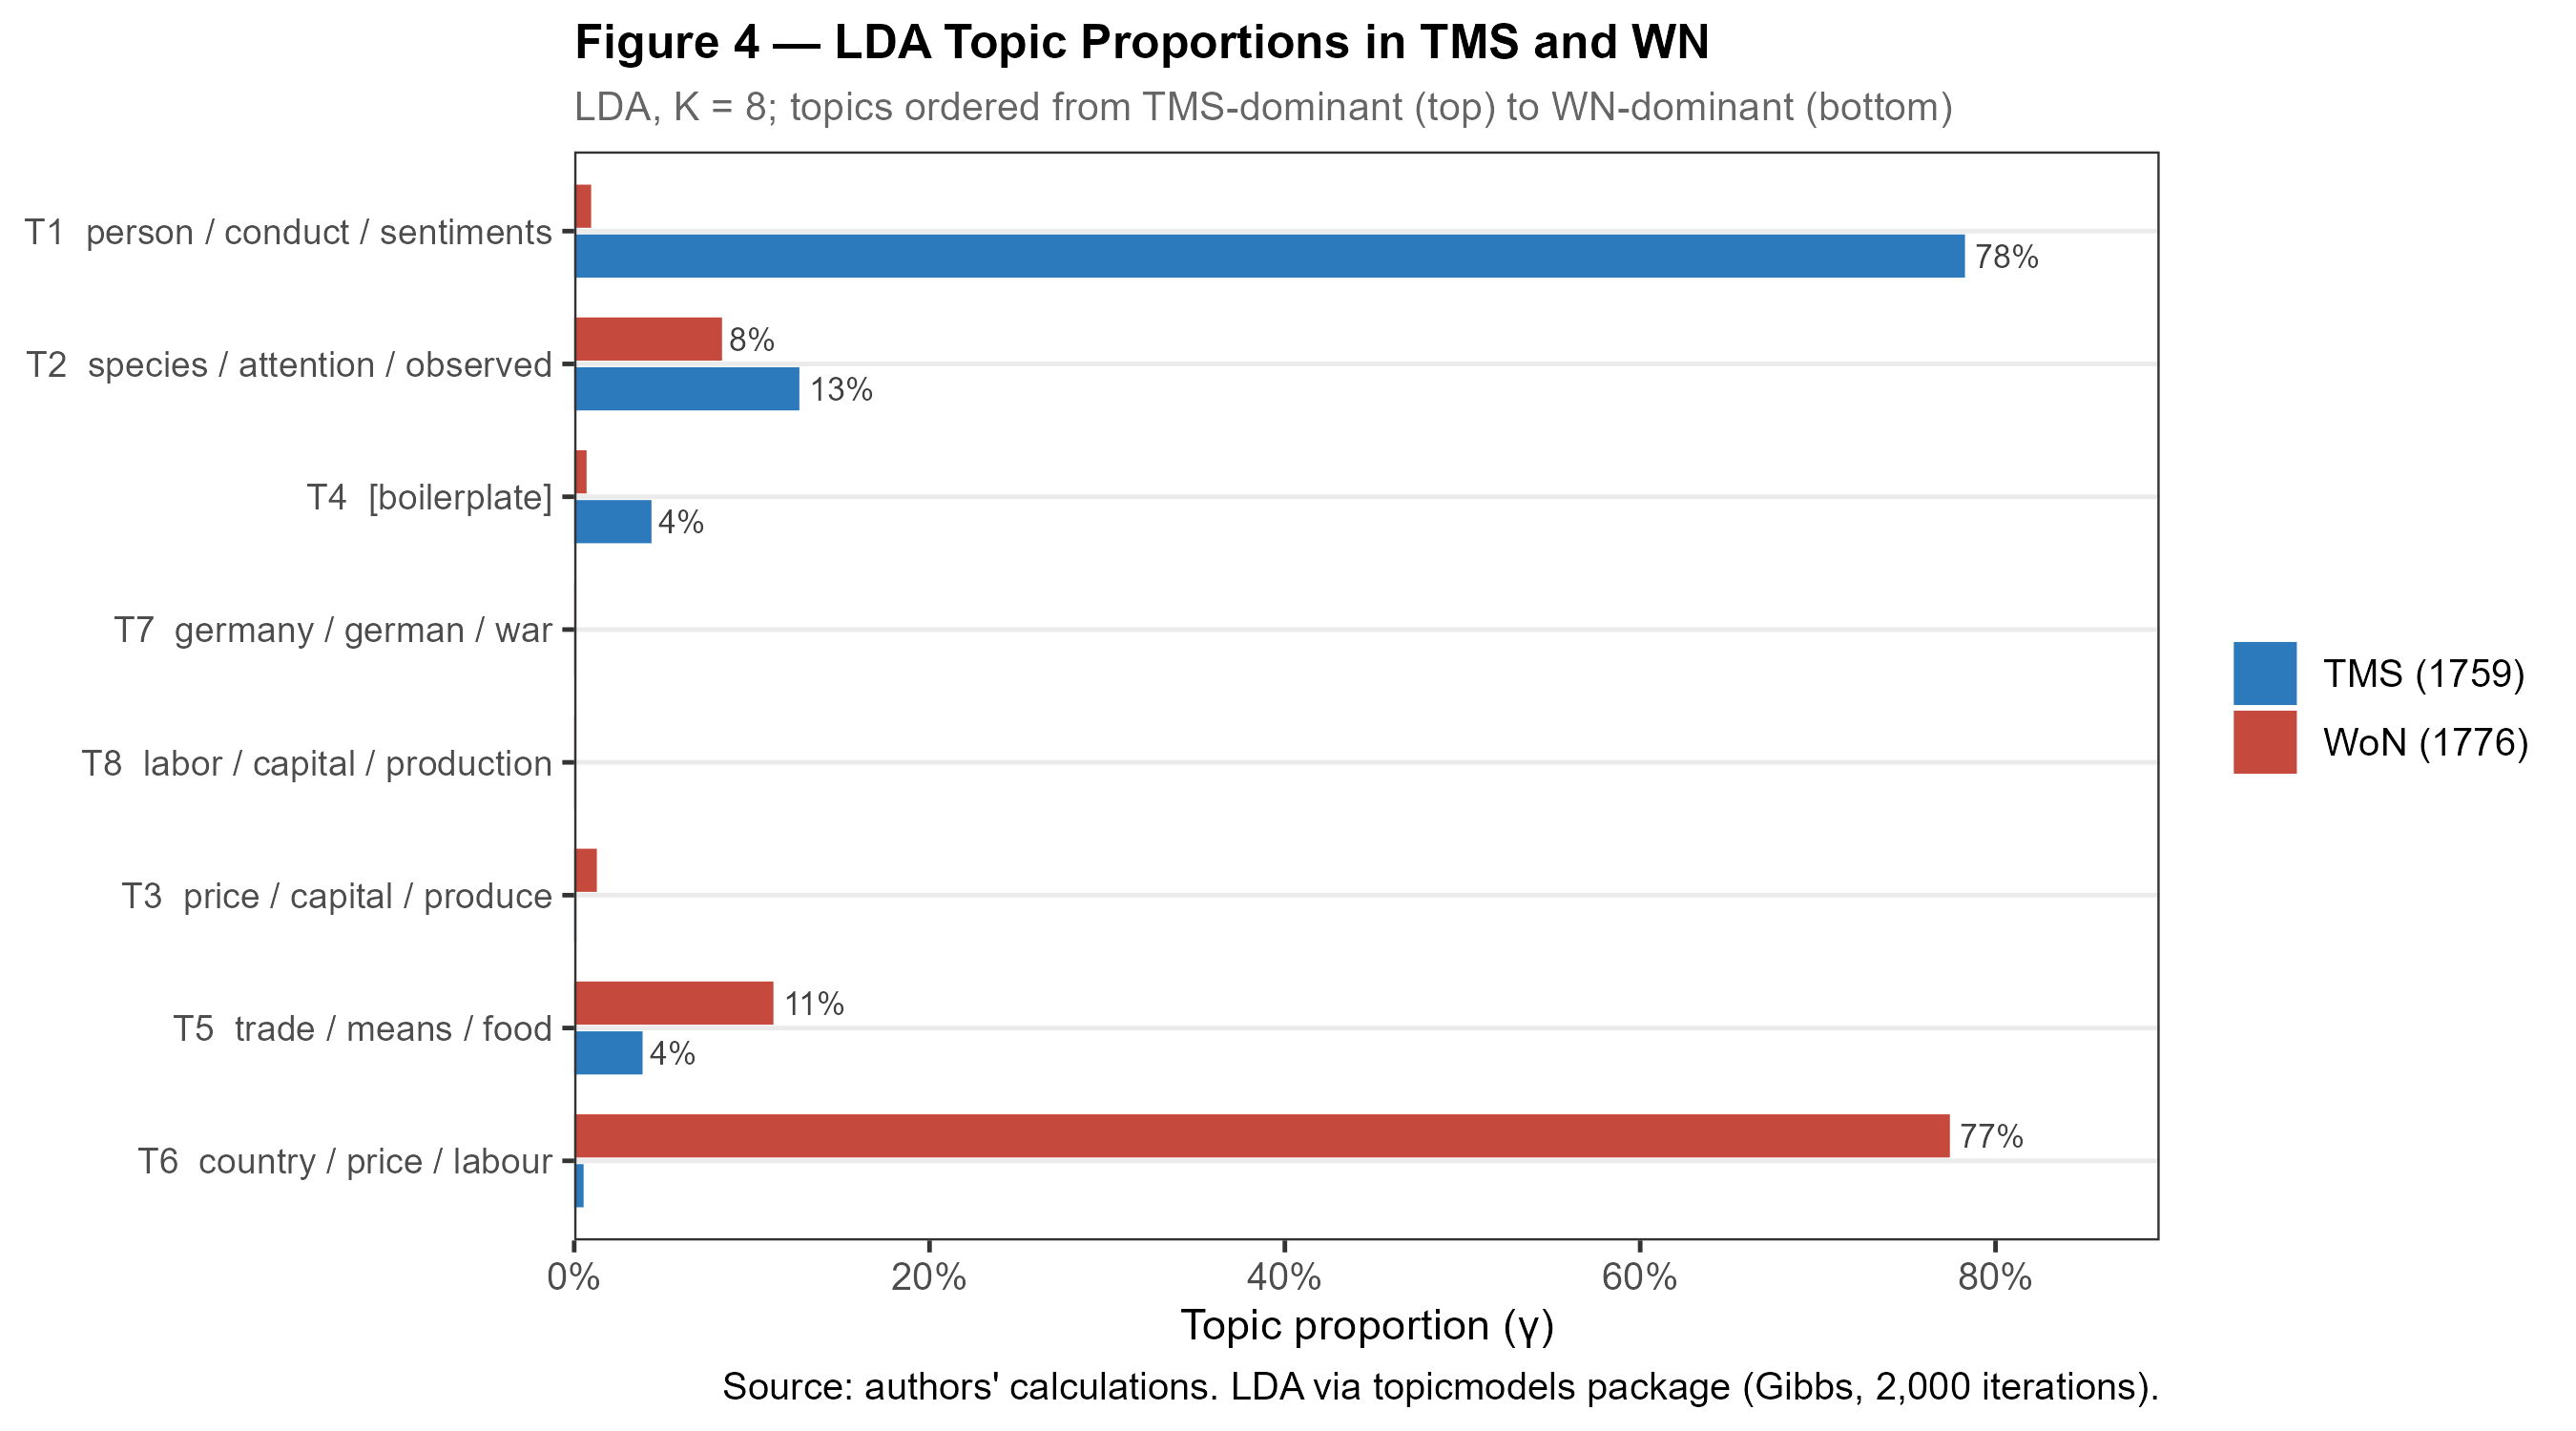
\includegraphics[width=\textwidth]{figuras/fig4_lda_topicos.png}
  \caption{LDA topic proportions ($\gamma$) in TMS and WN.
           $K = 8$; Gibbs sampling, 2,000 iterations.
           Topics ordered from TMS-dominant (top) to WN-dominant
           (bottom). Topic T4 captures Project Gutenberg boilerplate
           and is excluded from substantive interpretation.}
  \label{fig:lda}
\end{figure}

H5---Mixed result, supporting thematic separation with a shared
philosophical layer.
Topic T1 (``person / conduct / sentiments'') concentrates 78\% of
TMS's topic mass and less than 1\% of WN's.
Topic T6 (``country / price / labour'') concentrates 77\% of WN's
topic mass and less than 1\% of TMS's.
The thematic separation between the two works is near-complete at the
level of dominant topics.

However, Topic T2 (``species / attention / observed'') accounts for
13\% of TMS and 8\% of WN---a non-trivial shared loading.
This topic appears to capture the empiricist-observational idiom common
to Scottish moral philosophy: the careful observation of phenomena,
classification by species, and argumentation from observed regularities.
This layer is present in both works, suggesting that TMS and WN share
an underlying epistemological mode even as they diverge in object domain.
Appendix~B reports the full top-8-word lists for all topics.

Table~\ref{tab:hypotheses} summarizes all hypothesis results.

\begin{table}[H]
\centering
\caption{Summary of hypotheses and findings}
\label{tab:hypotheses}
\small
\begin{tabularx}{\textwidth}{llXl}
\toprule
Hyp. & Metric & Finding & Verdict \\
\midrule
H1 & lm\_positive & TMS: 0.0294 $>$ WN: 0.0239 & Confirmed \\
H2 & lm\_constraining & WN: 0.0110 $>$ TMS: 0.0086; chapter $p=0.09$ & Confirmed$^\dagger$ \\
H3 & lm\_uncertainty & WN $>$ TMS ($t=-3.35$; $p=0.001$) & Null rejected$^\ddagger$ \\
H4 & pct\_we / ratio\_we\_i & TMS: 2.12\% / 7.36 $\gg$ WN: 0.17\% / 1.52 & Confirmed \\
H5 & LDA $\gamma$ & T1 (moral) $\approx$ TMS only; T6 (econ.) $\approx$ WN only; T2 in both & Mixed \\
\midrule
\multicolumn{4}{l}{\small $^\dagger$ Directional at book level; below $p<0.05$ at chapter level.} \\
\multicolumn{4}{l}{\small $^\ddagger$ Null rejected, but WN more uncertain than TMS---reversal of intuitive prediction.} \\
\bottomrule
\end{tabularx}
\end{table}

% =============================================================
\section{Discussion}
% =============================================================

\subsection{On the Viability of Sentiment Analysis for Historical
Economic Texts}

The central methodological finding is that domain-appropriate sentiment
analysis \textit{is} viable for Smith's eighteenth-century prose.
The Jockers-Rinker dictionary failed not because sentiment analysis is
inapplicable to historical economic texts, but because its classifications
were calibrated for contemporary general language.
By substituting the LM dictionary, we obtain six attitudinal dimensions
that are theoretically interpretable and yield results consistent with
established scholarly knowledge about the two works.

This finding has implications for the field.
\citeauthor{Ballandonne2023} \citeyearpar{Ballandonne2023} identified
the correct source of the problem but drew too broad a conclusion.
Their recommendation to avoid sentiment analysis for historical economic
texts should be rephrased as: avoid \textit{generic} sentiment
dictionaries for domain-specific historical texts.
The appropriate correction is a domain-appropriate dictionary, not
methodological abstention.

The remaining limitation is coverage.
The LM dictionary covers 4,150 words derived from modern financial
prose; eighteenth-century vocabulary will include terms absent from LM
or present with different semantic weight.
This induces conservative bias---LM scores are lower bounds on
the true attitudinal loading of Smith's prose.
A productive agenda for future research would be to construct a
domain-and-period-specific dictionary for historical economic texts,
possibly by training a word embedding model on a broad corpus of
eighteenth- and nineteenth-century economic writing.

\subsection{Implications for the Adam Smith Problem}

Our results provide ammunition for both sides of the debate, though on
balance they favor the unity reading.

The LDA results (H5) show that the two works inhabit nearly disjoint
topic spaces at the level of dominant topics.
TMS's vocabulary orbits around persons, conduct, sentiments, and
virtue; WN's orbits around prices, labor, country, and trade.
The surface divergence is real.
If anything, the LDA result clarifies that \citeauthor{Ballandonne2023}
were right to describe TMS as ``topically'' different from WN.

The chapter-level uncertainty results (H3) support the unity reading
more strongly.
The standard dichotomy story implies that WN is the more scientific,
empirically precise work---the product of an enlightened political
economist who has moved beyond the speculative realm of moral sentiment.
Our finding reverses this: WN is the \textit{more hedged} text.
Smith in the political economy is epistemically cautious about market
phenomena; Smith in the moral philosophy speaks from a position of
greater rhetorical confidence.
This is consistent with \citeauthor{Evensky2005}'s reading that Smith
treated moral philosophy and political economy as complementary
enterprises operating at different levels of epistemic confidence:
the foundations of morality were relatively secure (universal sympathy,
natural desire for approbation); the mechanisms of market economies
were contingent and subject to revision.

The pronoun results (H4) add a further dimension.
The Smith of TMS addresses a ``we''---a community of moral agents who
share the capacity for sympathy and who jointly constitute the social
fabric of approbation.
The Smith of WN addresses the market impersonally, as a mechanism that
aggregates individual actions without requiring that actors recognize
each other as moral persons.
This difference in rhetorical mode does not imply a difference in
underlying moral philosophy: the market of WN operates \textit{within}
the social framework of mutual sympathy described in TMS.
The pronoun gap measures rhetorical register, not philosophical
contradiction.

\subsection{Limitations}

Four limitations deserve acknowledgment.
First, the corpus is small ($N = 2$ documents at the book level), which
prevents book-level statistical inference.
The chapter-level decomposition mitigates this but introduces noise from
uneven chapter lengths and the regularization fallback applied when
header detection finds fewer than five structural markers.

Second, the Gutenberg editions may differ from the critical editions
used by \citeauthor{Ballandonne2023} (Oxford Text Archive for TMS,
1784--86 Gutenberg for WN).
Edition differences could affect readability scores and vocabulary
coverage.
A robustness check using the critical Oxford Glasgow editions would
strengthen the comparisons with B\&C~(2023).

Third, Project Gutenberg files include standard license boilerplate
(header and footer text about the Gutenberg license and foundation).
This contaminates the corpus marginally---LDA Topic~T4 captures this
noise, confirming its presence.
Future analyses should apply systematic boilerplate stripping.

Fourth, the standard English stop-word list was not calibrated for
eighteenth-century prose.
Words such as ``shall,'' ``may,'' ``ought,'' and ``might'' sometimes
appear in modern stop-word lists but carry epistemic weight in Smith's
writing and are correctly retained by our pipeline; archaic forms
(``hath,'' ``doth,'' ``thee,'' ``thou'') may however be classified
inconsistently.
This is unlikely to affect the main findings materially, as the LM
dictionary matches on lemmatized content words, but a period-specific
stop-word list would be preferable.
Additionally, the LDA was trained on a six-text corpus that includes a
substantially truncated version of Knight (1921), which may affect topic
quality for non-Smith topics; the Smith-specific topics T1 and T6 are
robust given their high $\gamma$ concentrations.

% =============================================================
\section{Conclusion}
% =============================================================

This paper has demonstrated that the ``missing dictionary'' is the key
to unlocking productive sentiment analysis of Adam Smith's classical
texts.
\citeauthor{Ballandonne2023} correctly diagnosed the failure of the
Jockers-Rinker dictionary for economic prose but drew too broad a
conclusion.
By substituting the Loughran-McDonald dictionary, we obtain a rich
attitudinal profile of TMS and WN that is consistent with established
scholarly interpretation and yields a genuinely novel finding: WN
carries significantly more \textit{uncertainty} vocabulary than TMS at
the chapter level ($t = -3.35$; $p = 0.001$), a result that aligns with
the scholarly consensus against the dichotomy reading of the Adam Smith
Problem.

The first-person pronoun analysis independently confirms Brown's (1994)
dialogic/monologic distinction with a twelve-fold gap in ``we/our/us''
usage, formalizing a qualitative characterization as a testable index.
LDA topic modeling reveals near-perfect thematic separation at the level
of dominant topics, but also a shared Scottish empiricist idiom that
suggests intellectual continuity beneath the surface divergence.

The contributions to methodology are as important as the substantive
findings.
We establish that: (i) domain-appropriate dictionaries make sentiment
analysis viable for historical economic texts; (ii) topic modeling adds
a structural dimension missing from frequency-based approaches; and
(iii) chapter-level decomposition enables formal statistical inference
that is impossible at the book level.
These tools constitute a replicable protocol that can be applied to
other texts in the history of economic thought---a field that, as
\citeauthor{Ballandonne2023} argued, has yet to fully embrace the
quantitative turn.

Three directions for future research follow immediately.
First, extend the analysis to Smith's \textit{Lectures on
Jurisprudence} and \textit{Essays on Philosophical Subjects}, which
bridge the moral and economic projects.
Second, construct a period- and domain-specific sentiment dictionary for
eighteenth- and nineteenth-century economic prose, addressing the
coverage limitation identified here.
Third, apply the same protocol to contemporaries of Smith---Hume,
Hutcheson, Ferguson, and Ricardo---to contextualize Smith's rhetorical
choices within the broader tradition of Scottish Enlightenment thought.

% =============================================================
\bibliography{referencias}
\bibliographystyle{chicago}
% =============================================================

\newpage
\appendix

\section{Comparison: this paper vs.\ Ballandonne and Cersosimo (2023)}
\label{app:compare}

\begin{table}[H]
\centering
\caption{Methodological comparison: B\&C (2023) vs.\ this paper}
\label{tab:compare_bc}
\small
\begin{tabularx}{\textwidth}{lXX}
\toprule
Dimension & B\&C (2023) & This paper \\
\midrule
Software & R 4.1.3 + quanteda + sentimentr & R 4.2.3 + tidytext + topicmodels \\
Sentiment dict. & Jockers-Rinker (general) & Loughran-McDonald (economic) \\
Sent.\ categories & Positive/negative (1-D) & 6 dimensions \\
Topic modeling & Absent & LDA, K = 8 \\
Lexical richness & MATTR & --- \\
Readability & Flesch-Kincaid (main) & Flesch + FK + ARI \\
Pronouns & Raw frequencies & pct\_we, pct\_i, ratio\_we\_i \\
TF-IDF & Book level (2 docs) & Book level (2 docs) \\
Chapter analysis & Section/sentence (style) & Chapter (sentiment + tests) \\
Statistical tests & None & Welch's $t$-test (H2, H3) \\
Explicit hypotheses & Exploratory & 5 hypotheses, formally tested \\
\bottomrule
\end{tabularx}
\end{table}

\section{LDA Topic Words}
\label{app:lda}

\begin{table}[H]
\centering
\caption{Top 8 words per LDA topic ($K = 8$). LDA trained on 6-text corpus;
         columns show dominant Smith text and approximate loading for TMS and WN
         only. Topics T3, T5, T7, T8 are primarily loaded on non-Smith texts
         (T7: Keynes 1919; T8: Knight/Marshall); their TMS/WN loadings are
         residual.}
\small
\begin{tabular}{clp{8.5cm}}
\toprule
Topic & Smith loading & Top 8 words \\
\midrule
T1 & TMS~78\%, WN~$<$1\% & person, conduct, sentiments, nature, regard, virtue, object, propriety \\
T2 & TMS~13\%, WN~8\%    & species, attention, observed, command, render, derived, impossible, expected \\
T3 & non-Smith topic     & price, capital, produce, corn, rent, profits, commodities, quantity \\
T4 & TMS~4\%~(boilerplate) & \textit{[gutenberg, project, electronic, terms, copyright]} \\
T5 & non-Smith topic     & trade, means, food, property, paid, cost, found, low \\
T6 & WN~77\%, TMS~$<$1\% & country, price, labour, produce, trade, quantity, money, people \\
T7 & non-Smith (Keynes)  & germany, german, war, treaty, allies, europe, economic, france \\
T8 & non-Smith (Knight)  & labor, capital, production, money, wages, cost, united, country \\
\bottomrule
\end{tabular}
\end{table}

\end{document}
